%chktex-file 36
%chktex-file 23
%chktex-file 10
%chktex-file 17
%chktex-file 9
\documentclass[computationalMathematics.tex]{subfiles}

\begin{document}

%%%%%%%%%%%%%%~~~~~~~~~~~~~~~~~~~~~~~~~~~~~~~~~~~~~~~~%%%%%%%%%%%%%%%
\section{21st of September 2018 --- A. Frangioni}
%%%%%%%%%%%%%%~~~~~~~~~~~~~~~~~~~~~~~~~~~~~~~~~~~~~~~~%%%%%%%%%%%%%%%

\subsection{Mathematical background for optimization problems}

\begin{definition}[Minimum problem]\label{def:min_prob}
  Let $X$ be a set, called \textbf{feasible region} and let $f : X \to \R$ be \emph{any} function, called \textbf{objective function} we call \textbf{problem} the following
\[
  (P) \qquad f_* = \min \{f(x)~:x \in X\}
\]
\end{definition}


\begin{definition}[Feasible solution]
  Let $x \in F$ be a solution of the minimum problem in which the domain is a superset of $X \subset F$. 
  We say that $x$ is a \textbf{feasible solution} if $x \in X$.
  On the other hand, $x$ is \textbf{unfeasible} if $x \in F~\setminus~X$.
\end{definition}

\begin{definition}[Optimal solution]
  Under the same hypothesis of the above definition, we define $x_*$ such that $f(x_*) = f_*$ an \textbf{optimal solution}, where $f_* \leq f(x) \, \forall x \in X$, $\forall v > f_* \, \exists \, x \in X$ s.t.~$f(x) < v$.
\end{definition}

It is possible to find problems where there is no optimal solution at all.

\begin{example}
  There are two cases in which it is not possible to find an optimal solution:
  \begin{enumerate}
    \item The domain is empty, which may be not trivial to prove, since it is an NP-hard problem sometimes;
    \item We want to find the minimum of the objective function but it is unbounded below (\,$\forall M \, \exists x_M \in X$
      s.t.~$f(x_M) \leq M$\,).
      On the other hand, we need to maximize the function, but it is unbounded above.
  \end{enumerate}
\end{example}

\noindent We can now rewrite the problem of solving an optimization problem as:
\begin{enumerate}
  \item Finding $x_*$ and proving it is optimal
  \item Or proving $X = \emptyset$
  \item Or constructively prove $\forall M \, \exists x_M \in X$ s.t.~$f(x_M) \leq M$.
\end{enumerate}

Typically “$x \in \R$” actually mean “$x \in \mathbb{Q}$” with up to k digits precision and most of the times we consider optimal a solution which is close to the true optimal value, modulo some error ($\bar{x}$, the approximately optimal).

\begin{definition}[Absolute error]
  We call \textbf{absolute error} the gap between the real value and the one we obtained. Formally,
\[
  f(\bar{x}) - f_* \leq \varepsilon
\]
\end{definition}

\begin{definition}[Relative error]
  We define as \textbf{relative error} the absolute error, normalized by the true value of the function
\[
  ( \, f(\bar{x}) - f_* \, ) / | \, f_* \, | \leq \varepsilon
\]
\end{definition}

\noindent \textbf{Multi-objective Optimization}:\\
What happens if we have more than one objective function?\newline
Often you need more than one, say:
\[
  (P) \qquad \min \{[f_1(x),f_2(x)]~:x \in X\}
\]
with $f_1$, $f_2$ contrasting and/or with incomparable units (apples vs. oranges)

In multi-objective optimization, there does not typically exist a feasible solution that minimizes all objective functions simultaneously. Therefore, attention is paid to \emph{Pareto optimal solutions}; that is, solutions that cannot be improved in any of the objectives without degrading at least one of the other objectives.
\begin{definition}[Pareto frontier]
   A feasible solution $x^{1} \in X$is said to (Pareto) dominate another solution $x^{2} \in X$, if
  \[
  f_{i}(x^{1})\leq f_{i}(x^{2})\quad for\quad all\quad indices\quad i \in \{ 1,2,\dots ,k\}\quad and
\]
\[
  f_{j}(x^{1})\leq f_{j}(x^{2})\quad for\quad all\quad indices\quad j \in \{ 1,2,\dots ,k\}
\]
A solution $x^{*}\in X$ (and the corresponding outcome $f(x^{*})$) is called Pareto optimal, if there does not exist another solution that dominates it. The set of Pareto optimal outcomes is often called the \textbf{Pareto frontier}.
\end{definition}

\addpic{0.5}{pics/21sett/paretofront.png}{An example of Pareto frontier}{fig:21sett1}
\newpage
We are provided with two practical solutions:

\begin{description}
  \item[{\sc Scalarization:}] using a linear combination of the two functions: $f(x) = \alpha f_1(x) + \beta f_2(x)$;
  \addpic{0.4}{pics/21sett/scalar.png}{Maximize risk-adjusted return, $\min \{f_{1}(x) + \alpha f_{2}(x) ~:x \in X\}$}{fig:21sett1}
  \item[{\sc Budgeting:}] $f(x) = f_1(x)$, $X := X \cup \{ \, f_2(x) \leq b \, \}$, which intuitively corresponds to taking into account only one objective function and add the others as constraints, provided that the values of the other functions are not too high.
  \addpic{0.4}{pics/21sett/budget2.png}{Maximize return with budget on maximum risk, $\min \{f_{1}(x)~: f_{2}(x) \leq \beta ~:x \in X\}$}{fig:21sett1}
  \addpic{0.4}{pics/21sett/budget1.png}{Minimize risk with budget on minimum return,, $\min \{f_{2}(x)~: f_{1}(x) \leq \beta ~:x \in X\}$}{fig:21sett1}
\end{description}

\subsubsection{Examples of “Bad” optimization problems}
Here some problems that has no optimal solution:
\begin{itemize}
    \item empty case ($X = \emptyset$): $\min\{ x \; : \; x \in \R \land x \leq -1 \land x \geq 1\}$
    \item unbounded [below]:  $\min\{ x \; : \; x \in \R \land x \leq 0\}$
    \item bad $X$:  $\min\{ x \; : \; x \in \R \land x > 0\}$
    \item bad $f$ and  $X$:  $\min\{ x \; : \; x \in \R \land x > 0\}$
    \item bad $f$: let us consider an iterative algorithm that moves towards the optimum.
It may happen that the function decreases and increases along a certain direction but its non-continuity leads to the impossibility of reaching the optimum.
As an example, let us take the following

\[
  \min \left\{f(x) =\bigg\{\begin{array}{ll} x & \mbox{ if } x > 0 \\
        1 & \mbox{ if } x = 0
        \end{array} \; \; : \; \; x \in [0, 1]\right\}
\]
\end{itemize}
\newpage
\subsection{Infima, suprema and extended reals}
\noindent Since we minimize/maximize stuff, infima/suprema are important:
\begin{definition}[Totally ordered set]
  We say that  set $X$ is \textbf{totally ordered} if $\forall \, x, y \in X$, either $f(x) \leq f(y)$ or $f(y) \leq f(x)$.
\end{definition}

\begin{definition}[Infima and suprema]
  Given a totally ordered set $R$ and one of its subsets (say $S \subseteq R$)
\[
  s\text{ is the {\bf infimum} of } S \Leftrightarrow \underline{s} = \inf S
  \quad\Leftrightarrow\quad
  \underline{s} \leq s \;\; \forall s \in S
  \;\;\wedge\;\;
  \forall t > \underline{s} \; \exists \, s \in S \mbox{ s.t. } s \leq t
\]
\[
  s \text{ is the {\bf supremum} of } S \Leftrightarrow \bar{s} = \sup S
  \quad\Leftrightarrow\quad
  \bar{s} \geq s \;\; \forall s \in S
  \;\;\wedge\;\;
  \forall t < \bar{s} \; \exists \, s \in S \mbox{ s.t. } s \geq t
\]
\end{definition}

\noindent \textbf{Issue}: inf S/sup S may not exist in $\R$

\begin{definition}[Extended real]
  In the case of unbounded functions the value of infima or suprema are $\infty$, and we call \textbf{extended reals} $\overline{\R} = {-\infty} \cup \R \cup {+\infty}$.
\end{definition}

\begin{itemize}
    \item For all $S \subseteq \R, \sup / \inf S \in \overline{\R}$
    \item $\inf S = -\infty $ just a convenient notation for “there is no (finite) inf”
    \item $\inf \emptyset = \infty$, $\sup \emptyset = -\infty$
\end{itemize}

\subsection{(Monotone) Sequences in $\R$ and optimization}
\noindent We are interested in studying sequences, because iterative methods start from a certain point and move towards the optimal, hopefully.\\

Sequence of iterates $\{ x_i \} \subset X$ and $v_i = f ( x_i )$. Typically we can’t get $f_∗$ in finite time ($\exists i v_i = f_∗$), but we can
“get as close as we want”: there in the limit.


\begin{definition}[Limit]
  Given a sequence $\{ x_i \}$ the \textbf{limit} for $i \to \infty$ is defined as
\[
  \lim_{i \to \infty} v_i = v ~ \iff ~ \forall \varepsilon > 0 ~ \exists ~ h \text{ s.t. } \abs{v_i - v} \leq \varepsilon ~ \forall i \geq h
\]
\end{definition}

It may happen that a sequence has or does not have a limit. For example $\{ \frac{1}{n}\}$ has limit $0$ for $n \to +\infty$, while $\{ {(-1)}^n \}$ does not.

\begin{proposition}
  Let us be given a monotone sequence, then the sequence \textbf{does} have a limit.
\end{proposition}

Notice that given a sequence either it is monotone or it can be ``split'' into two monotone sequences (for example $\{ {(-1)}^n\}$ can be transformed into $\{ {(-1)}^{2n}\}$ and $\{ {(-1)}^{2n+1}\}$ and these two sequences are both monotone).\\

The obvious way to make $\{ vi \}$ monotone: keep aside the best
\[
    v_i^* = \min \{v_h: h\leq i\} \qquad \text{(best value at interaction i)}
\]

\begin{itemize}
    \item  $v_1^* \geq v_2^* \geq v_3^* \geq \, \dots \, \Rightarrow v_\infty^* = \lim_{i \to \infty} v_i^* \geq f_*$ ∗ (asymptotic estimate)
    \item $\lim_{i \to \infty} v_i^* = v_\infty^* = f_* \Rightarrow \{v_i\}$ minimizing sequence (of values)
\end{itemize}

\begin{figure}
    \centering
    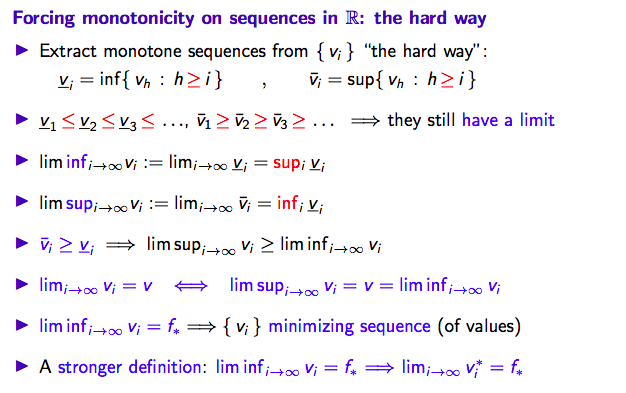
\includegraphics[scale = 0.6]{pics/21sett/forcing_monotonicity.png}
    \caption{Forcing monotonicity on sequences in $\R$: the hard way}
\end{figure}


\subsection{Vector spaces and topology}
\subsubsection{Euclidean space $\R^n$}
Single numbers are not enough, except for objective function values.
\begin{definition}[Euclidean vector space]
We call \textbf{Euclidean space}
\[
  \R^n := \{ \, \begin{pmatrix}x_1\\ x_2\\ \vdots\\ x_n\end{pmatrix}~:~x_i \in \R,~i = 1, \ldots, n\}
\]
Equivalently, we can characterize the Euclidean space as Cartesian product of $\R$ $n$ times: $\R^n = \R \times \R \times \ldots \R$. Closed under sum and scalar multiplication
\end{definition}

The main operations on elements of the Euclidean space (vectors) are:

\begin{description}
  \item[{\sc Sum:}] $x + y := \begin{pmatrix}x_1 + y_1\\
      x_2 + y_2\\
      \vdots\\
      x_n + y_n\\
  \end{pmatrix}$
\item[{\sc Scalar multiplication:}] $\alpha x = \begin{pmatrix}\alpha x_1\\
    \alpha x_2\\
    \vdots\\
    \alpha x_n\\
  \end{pmatrix}$
\end{description}

Usually $x \in \R^n$ usually considered “column vector” $\in \R^{n \times 1}$, otherwise a row vector is  $x^T$.

\begin{definition}[Finite vector space] each $x \in \R^n$ can be obtained from a finite basis. (canonical base is $u_i$ having 1 in position $i$ and 0 elsewhere)
\end{definition}
Notes for vector space:
\begin{itemize}
    \item Not all vector spaces are finite
    \item Not a totally ordered set
\end{itemize}

\noindent Concept of “limit” requires topology. So, in order to be able to compute limits in a vector space we need some topology definitions: norm, scalar product,  distance.\\


\subsubsection{(Euclidean) norm}
\begin{definition}
 Let $x \in \R^n$ we define the \textbf{euclidean norm} of a vector:
 $$\norm{x}_2 = \sqrt{\sum\limits_{i=1}^n {x_i}^2} = \sqrt{ \ps{x}{x}}$$
\end{definition}

\begin{proposition}
The norms on a vector space have the following properties:
\begin{enumerate}
  \item $\norm{x} \ge 0$ and $\forall x \in \R^n$, $\norm{x}=0~\iff~x=0$;
  \item $\norm{\alpha x} = \abs{\alpha} \norm{x},~\forall x \in \R^n,~\alpha \in \R$;
  \item $\norm{x+y} \le \norm{x} + \norm{y},~\forall x,y \in \R^n$ (triangle inequality).
\end{enumerate}
\end{proposition}

\begin{proposition}[Cauchy-Schwartz inequality]
  Let $x, y \in \R^n$. The following holds:
  \[
    \ps{x}{y}^2 \;\leq \; \ps{x}{x}\ps{y}{y}\equiv \abs{\ps{x}{y}} \leq \norm{x} \norm{y},~\forall x,y \in \R^n
  \]
\end{proposition}

\begin{proposition}[Parallelogram Law]
$$ 2\norm{x}^2 + 2\norm{y}^2 = \norm{x + y}^2 + \norm{x - y}^2$$
\end{proposition}

\begin{proposition}
$$ \norm{x + y}^2 = \norm{x}^2 + \norm{y}^2 + 2\ps{x}{y}$$
\end{proposition}


\subsubsection{A useful norm generalization: p-norm}
Many (but not all) derive from p-norm:
\begin{definition}[p-norm] Let $p \geq 1$ be a real number, the p-norm of a vector $x = ( x_1, \dots , x_n )$ is defined as follow:
$$ \norm{x}_p := \left( \sum_{i = 1}^n \abs{x_i}^p\right)^{1/p} $$
We require $p \geq 1$ for the general definition of the p-norm because the
triangle inequality fails to hold if $p < 1$.  The p-norm is convex for $p \geq 1$, nonconvex for $p < 1$
\end{definition}
Here some norm derived from p-norm:
\begin{itemize}
    \item $\norm{x}_1 := \sum_{i = 1}^n \abs{x_i}$
    \item $\norm{x}_\infty := \max\{ \abs{x_i}\; :\; i = 1, \dots, n \}$
    \item $\norm{x}_i := \abs{\{ i \; : \; \abs{x_i} > 0\}}$
    \item Other ones (e.g. for matrices . . . )
\end{itemize}
\begin{proposition}
For any given finite-dimensional vector space $V$ (e.g. $\R^n$ is a finite vector space), all norms on $V$ are equivalent in the sense that given two norms $\norm{\cdot}_A\, ,\,\norm{\cdot}_B$:
$$ \exists \; 0 < \alpha < \beta \;\; s.t\;\; \alpha\norm{x}_A \leq \norm{x}_B \leq \beta\norm{x}_A \qquad \forall x \in V$$
Therefore convergence in one norm implies convergence in any other norm. This rule
may not apply in infinite-dimensional vector spaces such as function spaces, though
\end{proposition}
\begin{proposition}[(Holder’s inequality]
$$ \ps{x}{y}^2 \leq \norm{x}_p\norm{y}_q \; \; 1/p + 1/q = 1$$

\end{proposition}

\begin{definition}[Ball]
We term \textbf{ball} centered in $\bar{x}$ and having $\varepsilon$ as radius as the set of points that are close enough to $x \in \R^n$: $B(\bar{x}, \varepsilon) = \{x \in \R^n~:~ \norm{x - \bar{x}} \le \varepsilon\}$.
\end{definition}

Let's take a unit ball, if the center of the unit-ball is in the origin (0,0), then each point on the unit-ball will have the same p-norm (i.e. 1). The unit ball therefore describes all points that have "distance" 1 from the origin, where "distance" is measured by the p-norm.
In \Cref{fig:21sett1} we may observe the different shapes of the same ball varying the value of $p$ in the $p$-norm.\\

\addpic{0.4}{pics/21sett/pnorms.pdf}{The shapes of balls centered in the origin of radius $1$ varying the value of $p$-norm.}{fig:21sett1}


\subsubsection{(Euclidean) Scalar Product}

\begin{definition}[Scalar product]
  Let $x, y \in \R^n$ we define the \textbf{scalar product} between these two vectors 
  \[
\ps{x}{y} \; := \; y^T x = \sum_{i=1}^n x_i y_i = x_1 y_1 + \cdots + x_n y_n
  \]
\end{definition}

\begin{proposition}
A scalar product has the following properties:
\begin{enumerate}
  \item $\ps{x}{y} = \ps{y}{x} \quad \forall x, y \in \R^n$ (symmetry)
  \item $\ps{x}{x} \ge 0,~\forall x \in \R^n$, $\ps{x}{x}=0~\iff~x=0$;
  \item $\ps{\alpha x}{y} = \alpha \ps{x}{y},~\forall x\in\R^n, \alpha \in \R$;
  \item $\ps{x + y}{z} = \ps{x}{z} + \ps{y}{z},~\forall x,y, z \in \R^n$.
\end{enumerate}
\end{proposition}

Geometric interpretation of the scalar product, an important characterization of the scalar product is the one that uses angles:
$$\ps{x}{y} = \norm{x} \norm{y} \cos \theta$$ 
\begin{itemize}
    \item $x \perp y \iff \ps{x}{y} = 0$ (orthogonality condition)
    \item $\ps{x}{y} \; >\;  0 \iff$ ``$x$ and $y$ point in the same direction''
\end{itemize}

\noindent More General: $ \ps{x}{y}_M := y^TMx $ with $M \succ 0$  $( x \longrightarrow M^{-1/2}x)$

\subsubsection{(Euclidean) Distance}
\begin{definition}[(Euclidean) distance]
The \textbf{Euclidean distance} between points $x$ and $y$ is the length of the line segment connecting them. In Cartesian coordinates, if $x = (x_{1}, x_{2},..., x_{n})$ and $y = (y_{1}, y_{2},..., y_{n})$ are two points in Euclidean n-space, then the distance ($d$) from $x$ to $y$, or from $y$ to $x$ is given by
  \[
    d(x,y) := \lVert x - y \rVert = \sqrt{(x_{1} - y_{1})^{2} + ... + (x_{n} - y_{n})^{2}} 
  \]
  
\end{definition}
 
 \begin{proposition}
The distance has the following properties:
\begin{enumerate}
  \item $d(x,y) \geq 0  \; \forall x,y \in \R^n \; , \; d(x,y) = 0 \iff x = y$
  
  \item $d(\alpha x,0) = \abs{\alpha}d(x,0) \; \; \forall x \in \R^n \, , \, \alpha \in \R $
  
  \item $ d(x,y) \leq d(x,z) + d(z, y) \; \; \forall x,y,z  \in \R^n$ (triangle inequality)
\end{enumerate}
\end{proposition}

\subsection{Limit of a sequence in $\R^n$}
We have now all the tools to define the notion of limit of a sequence in $\R^n$.
\noindent\textbf{Limit of a sequence in $R^n$}

\begin{definition}[Limit of a sequence in the Euclidean space]
  Let $\{ x_i \} \subset \R^n$ be a sequence in $\R^n$. The \textbf{limit} of $\{x_i\}$ for $i \to +\infty$ is the following:
  \[
    \lim_{i \to \infty} x_i = x \equiv \{ x_i \} \to x
  \]
  \[
    \Updownarrow
  \]
  \[
    \forall \varepsilon > 0~\exists h~\text{s.t.}~d(x_i , x) \leq \varepsilon~\forall i \geq h
  \]
  \[
    \Updownarrow
  \]
  \[
    \forall \varepsilon > 0~\exists h~\text{s.t.}~x_i \in \mathcal{B}( x , \varepsilon ) \; \forall i \geq h
  \]
  \[
    \Updownarrow
  \]
  \[
    \lim_{i \to \infty} d( x_i , x ) = 0
  \]
\end{definition}
\noindent \textbf{Note}: 
\begin{itemize}
    \item Points of ${x_i}$ eventually all come arbitrarily close to $x$
    \item No obvious lim inf / lim sup ($\R^n$ is not totally ordered)
\end{itemize}
\end{document}
